% !TEX root = book.tex
\makecstitle
\thispagestyle{empty}
{\sf
\noindent
ART is a generalised parser generator which delivers parsers that produce a representation of all of the derivations $\Delta_i$ for a sentence $\sigma$ in a grammar $\Gamma$. For instance, this grammar generates a language with three strings one of which has two derivations.\\[1ex]
}
\noindent$\Gamma$ = 
\begin{verbatim}
S ::= X Y
X ::= `a `r | `a
Y ::= `r `t | `t
\end{verbatim}
$\sigma=${\tt art}
\hspace*{-4cm}
\parbox{10cm}{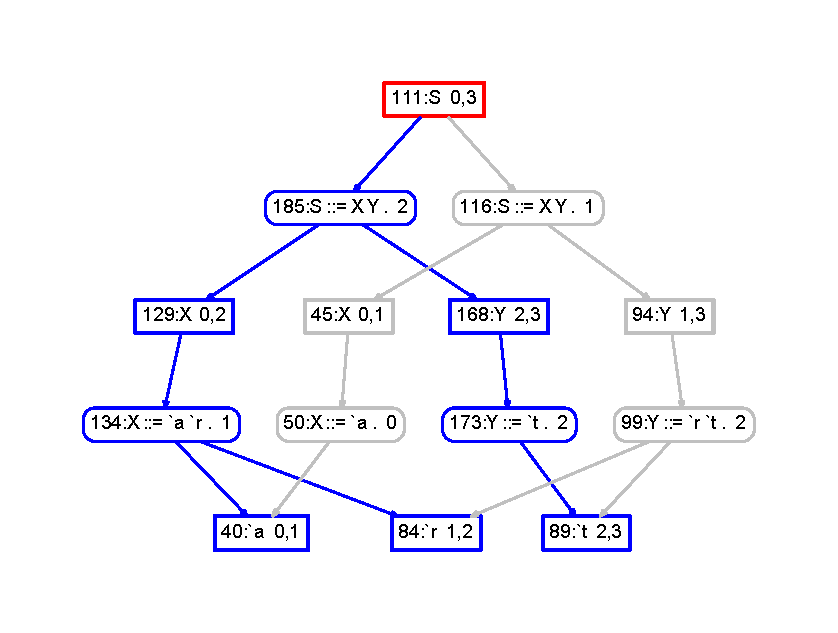
\includegraphics[width=10cm]{logo1.pdf}\\\hspace*{5.1cm}$\Delta_1$}
\parbox{10cm}{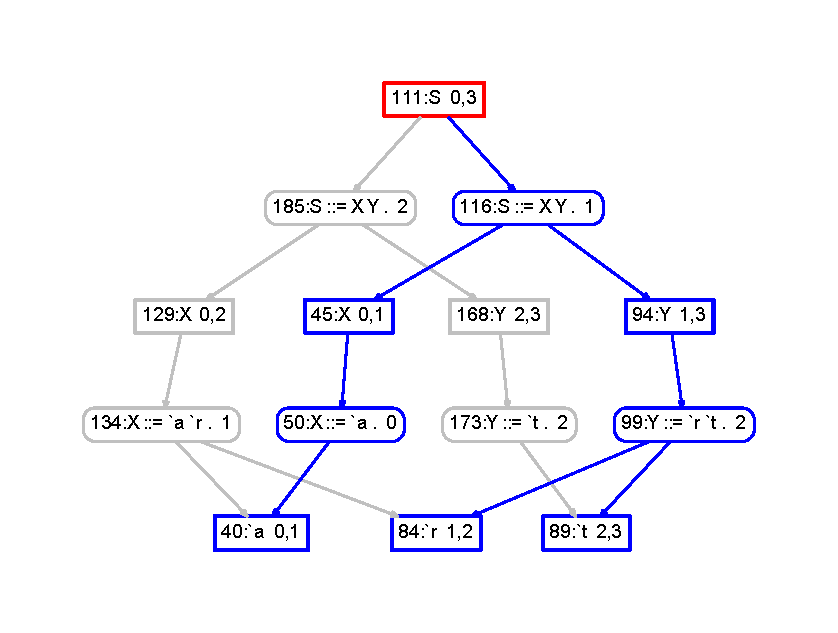
\includegraphics[width=10cm]{logo2.pdf}\\\hspace*{5.1cm}$\Delta_2$}\\[3ex]
{\sf
\noindent
As well as parsers, ART can generate ambiguity resolvers and abstract tree rewriters, along with evaluators for L-attributed grammars which may be used to make direct interpreters or translators to other languages. A limited form of higher order attributes is used to manage flow control in interpreters.\\[1ex]

\noindent
This document provides an introduction to the construction of programming language interpreters using ART.\\[1ex]

\noindent We develop a sequence of integer-only {\em Mini} languages introducing control flow via ART's delayed attributes.
We then turn to the handling of scopes and typing, implementing a dynamically typed language {\em Cava} with C/Java-like control structures. 

\noindent We finish with a domain specific language {\tt miniMusic} that allows melodies to be played using Java's built in MIDI synthesizer; there are many ways to improve miniMusic. A first step might be to add the domain specific elements to Cava\\[1ex]

\noindent{\small\bfseries The examples used in this tutorial are available in ARTInterpreterTutorial.zip, available from Royal Holloway's Centre for Software Language Engineering website.}}

\noindent{\sf Language interpreters in ART\ \ \copyright Adrian Johnstone and Elizabeth Scott 2017}
\clearpage
\setcounter{page}{1} \pagenumbering{roman} \tableofcontents
\cleardoublepage
